% =========================================================
% Metric Spaces — Notes Proofs Index
% =========================================================
% Dependency order:
%
% Level 0 — Pure metric (only metric axioms needed)
%   monotonicity-of-diameter     (def:diameter, sup comparison)
%   continuity-of-metric         (reverse triangle inequality)
%   convergence_preserved        (def:isometry, def:convergence)
%   preservation-of-diamter-in-isometry (def:isometry, def:diameter)
%
% Level 1 — Open sets (need balls + def:open-set)
%   union-open-sets              (def:open-set)
%   intersection-open-sets       (def:open-set, finiteness of min)
%
% Level 2 — Open/closed duality (need union-open, intersection-open)
%   closed-open                  (def:closed-set, def:open-set)
%   balls-open-closed            (radial gap, triangle inequality)
%
% Level 3 — Closed set operations (need closed-open + De Morgan)
%   intersection-closed-set      (closed-open, union-open)
%   finite-union-closed-sets     (closed-open, intersection-open)
%
% Level 4 — Closures and limit points
%   sequential-characterization-closure  (def:convergence, Archimedean)
%   proofs-limit-points                  (def:limit-point, sequential char)
%   equivalent-characterization-closure  (closure, seq char, balls-open-closed)
%
% Conceptual notes (not proofs, but inserted here for study):
%   openess   (conceptual distinction: openness vs completeness)
% =========================================================

% --- Level 0: Pure Metric ---
% =========================================================
% Proof: Monotonicity of Diameter
% Source: volume-iii/analysis/intro-metric-spaces/notes/notes-metric-space.tex
% Mode: standard
% =========================================================

\subsection*{Monotonicity of Diameter}
\label{prf:monotonicity-of-diameter}

\begin{remark*}[Return]
$\leftarrow$ \hyperref[thm:monotonicity-of-diameter]{Back to Theorem
(Monotonicity of Diameter) in Notes}
\end{remark*}

\begin{proof}
\Claim Let $(X, d)$ be a metric space and let $A \subseteq B \subseteq X$.
Then $\operatorname{diam}(A) \le \operatorname{diam}(B)$.

\Given A metric space $(X, d)$ and subsets $A \subseteq B \subseteq X$.
\Goal To show $\operatorname{diam}(A) \le \operatorname{diam}(B)$.
\Strategy We proceed directly by unfolding the definition of diameter and
using the fact that $A \subseteq B$ to bound the supremum over $A$ by
the supremum over $B$.

If $A = \varnothing$ then $\operatorname{diam}(A) = 0 \le \operatorname{diam}(B)$
and the result holds trivially. Assume henceforth that $A \neq \varnothing$.

\ByDef the diameter of a nonempty set $S \subseteq X$ is
\[
  \operatorname{diam}(S) \;=\; \sup\{\, d(x, y) \mid x, y \in S \,\}.
\]

\Let $x, y \in A$ be arbitrary.
Since $A \subseteq B$, we have $x, y \in B$, so $d(x,y)$ belongs to the
set $\{\, d(x,y) \mid x, y \in B \,\}$ over which $\operatorname{diam}(B)$
is taken.
\Therefore $d(x, y) \le \operatorname{diam}(B)$.

Since $x, y \in A$ were arbitrary, $\operatorname{diam}(B)$ is an upper
bound for $\{\, d(x,y) \mid x, y \in A \,\}$.
\ByThm{The supremum is the least upper bound}
$\operatorname{diam}(A) \le \operatorname{diam}(B)$. \AsReq
\end{proof}

\begin{remark*}[Proof shape]
Direct, with a one-line dispatch of the empty case. The subset inclusion
transfers pairs from $A$ into $B$, making $\operatorname{diam}(B)$ an upper
bound on pairwise distances in $A$; the least-upper-bound property of the
supremum then gives the inequality.
\end{remark*}

\begin{remark*}[Dependencies]
\begin{itemize}
  \item Definition of diameter:
        $\operatorname{diam}(S) = \sup\{d(x,y) \mid x, y \in S\}$
        \quad \ref{def:diameter}
  \item Convention: $\operatorname{diam}(\varnothing) = 0$
        \quad \ref{def:diameter}
  \item The supremum is the least upper bound: if $M$ is an upper bound
        for a set $S$ then $\sup S \le M$
        \quad \ref{thm:sup-least-upper-bound}
  \item Definition of subset:
        $A \subseteq B \Rightarrow (x \in A \Rightarrow x \in B)$
        \quad \ref{def:subset}
\end{itemize}
\end{remark*}
% =========================================================
% Proof: Continuity of the Metric
% Mode: standard
% =========================================================

\subsection*{Continuity of the Metric}
\label{prf:continuity-of-the-metric}

\begin{remark*}[Return]
$\leftarrow$ \hyperref[thm:continuity-of-metric]{Back to Theorem in Notes}
\end{remark*}

\begin{proof}
\Claim Let $(X,d)$ be a metric space. If $x_n \to x$ and $y_n \to y$ in $X$, then
$d(x_n, y_n) \to d(x, y)$ in $\mathbb{R}$.

\Given $x_n \to x$ and $y_n \to y$ in $(X,d)$.

\Goal To show $|d(x_n, y_n) - d(x, y)| \to 0$.

\Strategy Apply the reverse triangle inequality twice to bound
$|d(x_n, y_n) - d(x, y)|$ in terms of $d(x_n, x)$ and $d(y_n, y)$.

\medskip
\Strategy The key estimate: for all $n$,
\begin{align*}
|d(x_n, y_n) - d(x, y)|
&\le |d(x_n, y_n) - d(x, y_n)| + |d(x, y_n) - d(x, y)| \\
&\le d(x_n, x) + d(y_n, y).
\end{align*}
where the last step uses the reverse triangle inequality
(Proposition~\ref{prop:reverse-triangle}) twice:
\begin{align*}
|d(x_n, y_n) - d(x, y_n)| &\le d(x_n, x),\\
|d(x, y_n)  - d(x, y)|   &\le d(y_n, y).
\end{align*}

\medskip
\Let $\varepsilon > 0$.

\ByAss $x_n \to x$: $\exists N_1$ with $n \ge N_1 \Rightarrow d(x_n, x) < \varepsilon/2$.

\ByAss $y_n \to y$: $\exists N_2$ with $n \ge N_2 \Rightarrow d(y_n, y) < \varepsilon/2$.

\Let $N = \max(N_1, N_2)$.

For $n \ge N$:
\[
|d(x_n, y_n) - d(x,y)| \le d(x_n, x) + d(y_n, y) < \tfrac{\varepsilon}{2} + \tfrac{\varepsilon}{2} = \varepsilon.
\]

Since $\varepsilon > 0$ was arbitrary, $d(x_n, y_n) \to d(x, y)$. \AsReq
\end{proof}

\begin{remark*}[Proof shape]
Standard two-epsilon argument. The key tool is the reverse triangle inequality,
applied once per variable to replace $d(x_n, y_n)$ step-by-step with $d(x, y)$.
\end{remark*}

\begin{remark*}[Dependencies]
\begin{itemize}
  \item Proposition~\ref{prop:reverse-triangle}: $|d(u,z) - d(v,z)| \le d(u,v)$.
  \item Triangle inequality for $|\cdot|$ on $\mathbb{R}$.
  \item Definition of convergence in $(X,d)$ and in $(\mathbb{R}, |\cdot|)$.
\end{itemize}
\end{remark*}

% =========================================================
% Proof: Convergence is Preserved by Isometries
% Source: volume-iii/analysis/intro-metric-spaces/notes/notes-metric-space.tex
% Mode: standard
% =========================================================

\subsection*{Convergence is Preserved by Isometries}
\label{prf:convergence-preserved-by-isometry}

\begin{remark*}[Return]
$\leftarrow$ \hyperref[thm:convergence-preserved-by-isometry]{Back to Theorem
(Convergence is Preserved by Isometries) in Notes}
\end{remark*}

\begin{proof}
\Claim Let $(X,d_X)$ and $(Y,d_Y)$ be metric spaces and let
$f : X \to Y$ be an isometry.
If $(x_n)$ is a sequence in $X$ with $x_n \to x$ in $X$,
then $f(x_n) \to f(x)$ in $Y$.

\Given Metric spaces $(X,d_X)$ and $(Y,d_Y)$, an isometry
$f : X \to Y$, and a sequence $(x_n)$ in $X$ such that
$x_n \to x$.

\Goal To show that $f(x_n) \to f(x)$ in $Y$.

\Strategy We proceed directly by unfolding the definition of convergence
and using the defining property of an isometry.

Let $\varepsilon > 0$ be arbitrary. Since $x_n \to x$ in $X$,
there exists $N \in \mathbb{N}$ such that for all $n \ge N$,
\[
d_X(x_n, x) < \varepsilon.
\]

Since $f$ is an isometry, for all $n \in \mathbb{N}$ we have
\[
d_Y\bigl(f(x_n), f(x)\bigr) = d_X(x_n, x).
\]

Therefore, for all $n \ge N$,
\[
d_Y\bigl(f(x_n), f(x)\bigr) < \varepsilon.
\]

Hence $f(x_n) \to f(x)$ in $Y$. \AsReq
\end{proof}

\begin{remark*}[Proof shape]
Direct: fix $\varepsilon>0$, obtain $N$ from $x_n \to x$ in $(X,d_X)$, then
use distance preservation $d_Y(f(x_n),f(x))=d_X(x_n,x)$ to reuse the same $N$.
\end{remark*}

\begin{remark*}[Dependencies]
\begin{itemize}
  \item Definition of convergence of a sequence in a metric space.
  \item Definition of isometry.
\end{itemize}
\end{remark*}













% =========================================================
% Proof: Preservation of Diameter (Isometries)
% Mode: standard (stub)
% =========================================================

\subsection*{Preservation of Diameter}
\label{prf:preservation-of-diameter}

\begin{proof}
\Claim Let $(X,d_X)$ and $(Y,d_Y)$ be metric spaces and let
$f:X\to Y$ be an isometry. Then for every $A\subseteq X$,
\[
\operatorname{diam}(f(A))=\operatorname{diam}(A).
\]

\Given Metric spaces $(X,d_X)$, $(Y,d_Y)$, an isometry $f:X\to Y$, and a subset $A\subseteq X$.

\Goal To show $\operatorname{diam}(f(A))=\operatorname{diam}(A)$.

\Strategy Unfold the definition of diameter as a supremum of pairwise distances.
Use the defining property of an isometry to relate distances in $A$ to distances in $f(A)$.
Establish the needed set-inclusion(s) between the corresponding distance-sets and conclude equality of suprema.


Assume $f$ is an isometry, so
\[
d_Y\bigl(f(x),f(y)\bigr)=d_X(x,y)
\quad
\text{for all } x,y\in X.
\]

Let $x,y\in A$ be arbitrary.

Then the distance between their images equals the original distance:
\[
d_Y\bigl(f(x),f(y)\bigr)=d_X(x,y).
\]

\[
\begin{aligned}
\operatorname{diam}(A) &= \sup\{ d_X(x,y) : x,y \in A \} \\
\operatorname{diam}(f(A)) &= \sup\{ d_Y(f(x), f(y)) : x,y \in A \}.
\end{aligned}
\]

Since $d_Y(f(x),f(y)) = d_X(x,y)$ for all $x,y \in A$, we obtain
\[
\sup\{ d_Y(f(x), f(y)) : x,y \in A \}
=
\sup\{ d_X(x,y) : x,y \in A \}.
\]

Therefore
\[
\operatorname{diam}(f(A))=\operatorname{diam}(A).
\]
\end{proof}

\begin{remark*}[Dependencies]
\begin{itemize}
  \item Definition of isometry: $d_Y(f(x),f(y))=d_X(x,y)$ for all $x,y\in X$.
  \item Definition of image of a set: $f(A)=\{f(a):a\in A\}$.
  \item Definition of diameter: $\operatorname{diam}(A)=\sup\{d_X(x,y):x,y\in A\}$.
  \item Basic facts about $\sup$ and set inclusion (monotonicity of $\sup$).
\end{itemize}
\end{remark*}


% --- Level 1: Open Sets ---
% =========================================================
% Proof: Arbitrary Unions of Open Sets are Open
% Mode: standard
% =========================================================

\subsection*{Arbitrary Unions of Open Sets are Open}
\label{prf:union-open}

\begin{proof}
\Claim Let $(X,d)$ be a metric space and let $\{U_i\}_{i \in I}$
be any collection of open subsets of $X$.
Then $\bigcup_{i \in I} U_i$ is open.

\Given Open sets $U_i \subseteq X$ for $i \in I$.

\Goal To show $U := \bigcup_{i \in I} U_i$ is open: every point of $U$
has an open ball around it contained in $U$.

\Strategy An arbitrary point of $U$ must belong to at least one $U_i$.
The openness of that $U_i$ immediately provides the needed ball.

\medskip
\Let $x \in U$.

\ByDef of union: $\exists i_0 \in I$ such that $x \in U_{i_0}$.

\ByAss $U_{i_0}$ is open and $x \in U_{i_0}$: $\exists r > 0$ such that $B_r(x) \subseteq U_{i_0}$.

\ByDef of union: $U_{i_0} \subseteq U$.

\Therefore $B_r(x) \subseteq U_{i_0} \subseteq U$.

Since $x \in U$ was arbitrary, $U$ is open. \AsReq
\end{proof}

\begin{remark*}[Proof shape]
One step: a ball that fits inside some $U_{i_0}$ automatically fits inside
the union, since $U_{i_0} \subseteq \bigcup_i U_i$.
The argument works for \emph{arbitrary} (possibly infinite or uncountable) unions.
\end{remark*}

\begin{remark*}[Dependencies]
\begin{itemize}
  \item Definition~\ref{def:open-closed-set}: $U$ is open iff $\forall x \in U, \exists r > 0, B_r(x) \subseteq U$.
\end{itemize}
\end{remark*}

% =========================================================
% Proof: Finite Intersections of Open Sets are Open
% Mode: standard
% =========================================================

\subsection*{Finite Intersections of Open Sets are Open}
\label{prf:finite-intersection-open}

\begin{proof}
\Claim Let $(X,d)$ be a metric space and let
$U_1,\dots,U_n$ be open subsets of $X$.
Then $\bigcap_{k=1}^{n} U_k$ is open.

\Given A metric space $(X,d)$ and open sets $U_1,\dots,U_n \subseteq X$.

\Goal To show that $U := \bigcap_{k=1}^{n} U_k$ is open.

\Strategy Use the definition of open set:
take an arbitrary point in the intersection and use the openness
of each $U_k$ to construct a ball contained in all of them.

\medskip

Let $x \in U$ be arbitrary. Then $x \in U_k$ for each
$k = 1,\dots,n$.

Since each $U_k$ is open and $x \in U_k$, by the definition
of open set there exists $r_k > 0$ such that
\[
B(x,r_k) \subseteq U_k .
\]

Define
\[
r := \min\{r_1,r_2,\dots,r_n\}.
\]
Since the set $\{r_1,\dots,r_n\}$ is finite and each $r_k>0$,
we have $r>0$.

Let $y \in B(x,r)$. Then $d(x,y) < r \le r_k$ for each
$k = 1,\dots,n$. Hence $y \in B(x,r_k) \subseteq U_k$
for every $k$.

Therefore $y \in \bigcap_{k=1}^{n} U_k = U$.
Thus
\[
B(x,r) \subseteq U .
\]

Since $x$ was arbitrary, every point of $U$ has an open ball
contained in $U$. Therefore $U$ is open.
\end{proof}

\begin{remark*}[Dependencies]
\begin{itemize}
  \item Definition of open ball.
  \item Definition of open set.
  \item (Key idea) Use a minimum of finitely many radii.
\end{itemize}
\end{remark*}




% =========================================================
% TikZ: Finite Intersection of Open Sets is Open (U1, U2)
% Matches the picture: two big overlapping sets + three concentric balls
% "50% bigger" achieved via scale=1.5
% =========================================================

\begin{tikzpicture}[scale=1.5, line cap=round, line join=round]

  %--- Colors (close to your screenshot)
  \definecolor{Uone}{RGB}{58,103,190}   % blue stroke
  \definecolor{Utwo}{RGB}{176,94,52}    % brown/orange stroke

  %--- Centers/radii for the two sets (tweak overlap by changing their centers)
  \coordinate (c1) at (-2.3,0.0);   % move right/left to adjust overlap
\coordinate (c2) at ( 1.9,0.0);
   % move left/right to adjust overlap
  \def\Rset{2.25}

  %--- Point x in the overlap
  \coordinate (x) at (0.0,0.0);

  %--- Radii for the balls around x
  \def\rmin{1.05}   % r = min{r1,r2}
  \def\rone{1.25}   % r1
  \def\rtwo{1.70}   % r2

  %--- Title
  \node at (0,2.85) {$r=\min\{r_1,r_2\}$};

  %--- Fill the open sets (light)
  \fill[Uone!12] (c1) circle (\Rset);
  \fill[Utwo!12] (c2) circle (\Rset);

  %--- Boundaries of U1, U2
  \draw[Uone, line width=0.9pt] (c1) circle (\Rset);
  \draw[Utwo, line width=0.9pt] (c2) circle (\Rset);

  %--- Labels for U1, U2
  \node[Uone] at ($(c1)+(0,1.35)$) {$U_1$};
  \node[Utwo] at ($(c2)+(0,1.35)$) {$U_2$};

  %--- Balls around x
  \draw[black, dashed, line width=0.7pt] (x) circle (\rtwo);
  \draw[black, dashed, line width=0.7pt] (x) circle (\rone);
  \draw[black, line width=0.8pt]         (x) circle (\rmin);

  %--- Point x and a radius segment labeled r
  \fill[black] (x) circle (1.2pt);
  \node[above right] at (x) {$x$};

  \draw[black, line width=0.5pt] (x) -- ++(25:\rmin);
  \node at ($(x)+(25:0.62*\rmin)$) {\scriptsize $r$};

  %--- Labels for the balls (positions chosen to mimic your screenshot)
  \node at (-0.95, 0.20) {$B(x,r_1)$};
  \node at ( 0.95,-0.15) {$B(x,r_2)$};
  \node at ( 0.00,-1.15) {$B(x,r)$};

  %--- Intersection label
  \node at (0.00,-0.65) {$U_1\cap U_2$};

\end{tikzpicture}















% --- Level 2: Open/Closed Duality ---
% =========================================================
% Proof: Closed iff Complement Open
% Mode: standard
% =========================================================

\subsection*{Closed Sets and Open Complements}
\label{prf:closed-iff-complement-open}

\begin{remark*}[Return]
$\leftarrow$ \hyperref[thm:closed-iff-complement-open]{Back to Theorem
(Closed iff Complement Open) in Notes}
\end{remark*}

\begin{proof}
\Claim Let $(X,d)$ be a metric space and $F \subseteq X$.
$F$ is closed (i.e.\ $F$ contains all limits of sequences in $F$)
if and only if $X \setminus F$ is open.

\Given A metric space $(X,d)$ and $F \subseteq X$.

\Goal To prove $F$ closed $\Longleftrightarrow$ $X \setminus F$ open.

\Strategy Both directions proceed by contraposition at the level of points:
a point outside a closed set has a ball keeping it outside;
a sequence in $F$ heading for the exterior contradicts closedness.

\medskip
\noindent\textbf{($\Rightarrow$) $F$ closed $\Rightarrow$ $X \setminus F$ open.}

\Let $y \in X \setminus F$. We must find $r > 0$ with $B_r(y) \subseteq X \setminus F$.

Suppose for contradiction that no such $r$ exists. Then for each $n \ge 1$,
$B_{1/n}(y)$ contains a point $x_n \in F$.
The sequence $(x_n)$ lies in $F$ and $d(x_n, y) < 1/n \to 0$, so $x_n \to y$.

\ByAss $F$ is closed: since $(x_n) \subseteq F$ and $x_n \to y$, we have $y \in F$.
This contradicts $y \in X \setminus F$. \Therefore the $r$ exists and $X \setminus F$ is open.

\medskip
\noindent\textbf{($\Leftarrow$) $X \setminus F$ open $\Rightarrow$ $F$ closed.}

\Let $(x_n) \subseteq F$ with $x_n \to x$.

Suppose for contradiction that $x \notin F$, so $x \in X \setminus F$.

\ByAss $X \setminus F$ is open: $\exists r > 0$ with $B_r(x) \subseteq X \setminus F$.

\ByAss $x_n \to x$: $\exists N$ with $n \ge N \Rightarrow d(x_n, x) < r$, i.e.\ $x_n \in B_r(x) \subseteq X \setminus F$.

But $x_n \in F$, so $x_n \in F \cap (X \setminus F) = \varnothing$. Contradiction.

\Therefore $x \in F$. Since the sequence $(x_n) \subseteq F$ was arbitrary, $F$ is closed. \AsReq
\end{proof}

\begin{remark*}[Proof shape]
Both directions use a sequence argument: build a sequence converging
to the relevant point and derive a contradiction if the conclusion fails.
\end{remark*}

\begin{remark*}[Dependencies]
\begin{itemize}
  \item Definition~\ref{def:open-closed-set}: $F$ closed means $F$ is sequentially closed.
  \item Definition~\ref{def:open-closed-set}: $U$ open means every point has a ball inside.
  \item Archimedean property: $1/n \to 0$.
\end{itemize}
\end{remark*}

% =========================================================
% Proof: Balls are open and closed
% Source: volume-iii/analysis/metric-spaces/notes/notes-balls.tex
% =========================================================

\subsection*{Balls are open and closed}
\label{prf:balls-open-closed}

\begin{remark}[Return]
\hyperref[prop:balls-open-closed]{$\leftarrow$ Back to Proposition (Balls are open and closed) in Notes}
\end{remark}

\begin{proposition}[Balls are open and closed]
Let $(X, d)$ be a metric space, $x \in X$, and $r > 0$.
\begin{enumerate}[label=(\roman*)]
  \item $B_r(x)$ is an open set.
  \item $\overline{B}_r(x)$ is a closed set.
\end{enumerate}
\end{proposition}

\begin{proof}
\Given A metric space $(X, d)$, a point $x \in X$, and a radius $r > 0$.
\Goal To show (i) $B_r(x)$ is open, and (ii) $\overline{B}_r(x)$ is closed.

\medskip
\noindent\textit{Part (i): $B_r(x)$ is open.}

\Strategy We show that every point of $B_r(x)$ has an open ball around it
still contained in $B_r(x)$.

Let $x_0 \in B_r(x)$.
By definition of open ball in a metric space,
\[
d(x,x_0) < r.
\]
Choose $\varepsilon>0$ with $\varepsilon < r - d(x,x_0)$. 
Claim $B_\varepsilon(x_0) \subseteq B_r(x)$.

Let $x_1 \in B_\varepsilon(x_0)$ be arbitrary. Then
\begin{align*}
d(x_0,x_1) &< \varepsilon,\\
d(x,x_1) &\le d(x,x_0) + d(x_0,x_1).
\end{align*}
Since $\varepsilon < r - d(x,x_0)$, we have $d(x,x_0) < r - \varepsilon$. Therefore,
\begin{align*}
d(x,x_1) 
&\le d(x,x_0) + d(x_0,x_1)\\
&< (r-\varepsilon) + \varepsilon\\
&= r.
\end{align*}
Hence, $x_1 \in B_r(x)$, and thus $B_\varepsilon(x_0) \subseteq B_r(x)$.

Since $x_1 \in B_\varepsilon(x_0)$ was arbitrary, it follows that
\[
B_\varepsilon(x_0) \subseteq B_r(x).
\]
Since $x_0 \in B_r(x)$ was arbitrary, every point of $B_r(x)$ admits an
$\varepsilon$-ball contained in $B_r(x)$. Therefore $B_r(x)$ is open.

\medskip
\noindent\textit{Part (ii): $\overline{B}_r(x)$ is closed.}

\Strategy We show that $X \setminus \overline{B}_r(x)$ is open, i.e.\ every
point outside the closed ball has an open ball around it disjoint from
$\overline{B}_r(x)$.

Let $x_0 \in X \setminus \overline{B}_r(x)$ be arbitrary. Then $d(x,x_0) > r$.

Choose $\varepsilon>0$ with $\varepsilon < d(x,x_0) - r$. 
Claim $B_\varepsilon(x_0) \subseteq X \setminus \overline{B}_r(x)$.

Let $x_1 \in B_\varepsilon(x_0)$ be arbitrary. Then
\begin{align*}
d(x_0,x_1) &< \varepsilon,\\
d(x,x_0) &\le d(x,x_1) + d(x_1,x_0).
\end{align*}

Since $\varepsilon < d(x,x_0) - r$, we have $\varepsilon + r < d(x,x_0)$. Therefore,
\begin{align*}
\varepsilon + r < d(x,x_0)
&\le d(x,x_1) + d(x_0,x_1)\\
&< d(x,x_1) + \varepsilon,
\end{align*}

which implies
\[
r < d(x,x_1).
\]

Hence $x_1 \notin \overline{B}_r(x)$, so
\[
B_\varepsilon(x_0) \subseteq X \setminus \overline{B}_r(x).
\]

Since $x_0 \in X \setminus \overline{B}_r(x)$ was arbitrary,
the complement of $\overline{B}_r(x)$ is open. Therefore
$\overline{B}_r(x)$ is closed.













\end{proof}

\begin{remark}[Proof shape]
% YOUR PROOF SHAPE HERE
\end{remark}

\begin{remark}[Dependencies]
\begin{itemize}
  \item Definition of open ball: \ref{def:open-ball}
  \item Definition of closed ball: \ref{def:closed-ball}
  \item Definition of open set: \ref{def:open-closed-set}
  \item Triangle inequality (metric axiom M4)
\end{itemize}
\end{remark}

% --- Level 3: Closed Set Operations ---
% =========================================================
% Proof: Intersection of Closed Sets is Closed
% Mode: standard
% =========================================================

\subsection*{Intersection of Closed Sets is Closed}
\label{prf:intersection-closed}

\begin{proof}
\Claim Let $(X,d)$ be a metric space and let $\{F_i\}_{i \in I}$ be any
collection of closed subsets of $X$. Then $\bigcap_{i \in I} F_i$ is closed.

\Given Closed sets $F_i \subseteq X$ for $i \in I$.

\Goal To show $F := \bigcap_{i \in I} F_i$ is closed.

\Strategy Use the complement characterization: $F$ is closed iff $X \setminus F$ is open.
By De Morgan's law, $X \setminus \bigcap_i F_i = \bigcup_i (X \setminus F_i)$,
an arbitrary union of open sets (since each $F_i$ is closed, $X \setminus F_i$ is open).
Arbitrary unions of open sets are open by Proposition~\ref{prop:union-open}.

\medskip
\ByAss each $F_i$ is closed, so each $X \setminus F_i$ is open.

\ByThm{De Morgan's law}:
\[
X \setminus F \;=\; X \setminus \bigcap_{i \in I} F_i \;=\; \bigcup_{i \in I} (X \setminus F_i).
\]

\ByThm{Proposition~\ref{prop:union-open}} an arbitrary union of open sets is open.

\Therefore $X \setminus F$ is open, so $F$ is closed. \AsReq
\end{proof}

\begin{remark*}[Proof shape]
De Morgan converts the intersection of closed sets into a union of open sets,
and arbitrary unions of open sets are open. The argument works for any
(finite, countable, or uncountable) collection.
\end{remark*}

\begin{remark*}[Dependencies]
\begin{itemize}
  \item Definition~\ref{def:open-closed-set}: $F$ closed $\iff$ $X \setminus F$ open.
  \item De Morgan's law: $X \setminus \bigcap_i F_i = \bigcup_i (X \setminus F_i)$.
  \item Proposition~\ref{prop:union-open}: arbitrary unions of open sets are open.
\end{itemize}
\end{remark*}

% =========================================================
% Proof: Finite Union of Closed Sets is Closed
% Mode: standard
% =========================================================

\subsection*{Finite Union of Closed Sets is Closed}
\label{prf:finite-union-closed}

\begin{proof}
\Claim Let $(X,d)$ be a metric space and let $F_1, \dots, F_n \subseteq X$ be closed.
Then $\bigcup_{k=1}^n F_k$ is closed.

\Given Closed sets $F_1, \dots, F_n \subseteq X$.

\Goal To show $F := \bigcup_{k=1}^n F_k$ is closed, i.e.\ $X \setminus F$ is open.

\Strategy Use the complement characterization and De Morgan's law.
The complement of a finite union is a finite intersection of open sets,
and finite intersections of open sets are open.

\medskip
\ByAss each $F_k$ is closed, so each $X \setminus F_k$ is open.

\ByThm{De Morgan's law}:
\[
X \setminus F \;=\; X \setminus \bigcup_{k=1}^n F_k \;=\; \bigcap_{k=1}^n (X \setminus F_k).
\]

\ByThm{Proposition~\ref{prop:finite-intersection-open}} a finite intersection of open sets is open.

\Therefore $X \setminus F$ is open, so $F$ is closed. \AsReq
\end{proof}

\begin{remark*}[Why finiteness is essential]
An infinite union of closed sets need not be closed.
For example in $\mathbb{R}$: $\{1/n\}$ is closed for each $n \ge 1$,
but $\bigcup_{n=1}^\infty \{1/n\} = \{1, 1/2, 1/3, \ldots\}$
is not closed: $0$ is a limit point not in the set.
\end{remark*}

\begin{remark*}[Dependencies]
\begin{itemize}
  \item Definition~\ref{def:open-closed-set}: $F$ closed $\iff$ $X \setminus F$ open.
  \item De Morgan's law: $X \setminus \bigcup_k F_k = \bigcap_k (X \setminus F_k)$.
  \item Proposition~\ref{prop:finite-intersection-open}: finite intersections of open sets are open.
\end{itemize}
\end{remark*}


% --- Level 4: Closures and Limit Points ---
% =========================================================
% Proof: Sequential Characterization of Closure Points
% Source: volume-iii/analysis/intro-metric-spaces/notes/notes-metric-space.tex
% Mode: standard (stub)
% =========================================================

\subsection*{Sequential Characterization of Closure Points}
\label{prf:sequential-characterization-closure}

\begin{remark*}[Return]
$\leftarrow$ \hyperref[thm:sequential-characterization-closure]{Back to Theorem
(Sequential Characterization of Closure Points) in Notes}
\end{remark*}

\begin{proof}
\Claim Let $(X,d)$ be a metric space, let $A \subseteq X$, and let $x \in X$.
There exists a sequence $(a_n)$ in $A$ such that $a_n \to x$
if and only if
\[
\forall r > 0,\quad B_r(x) \cap A \neq \varnothing.
\]

\Given A metric space $(X,d)$, a subset $A \subseteq X$, and a point $x \in X$.

\Goal To prove the equivalence:
\[
\bigl(\exists (a_n) \subseteq A \text{ with } a_n \to x\bigr)
\;\Longleftrightarrow\;
\bigl(\forall r>0,\; B_r(x)\cap A\neq\varnothing\bigr).
\]

\Strategy Prove both directions separately:

\medskip

\noindent
(\(\Rightarrow\)) Assume there exists a sequence $(a_n)\subseteq A$
with $a_n \to x$.
Use the definition of convergence to show that every ball
$B_r(x)$ must intersect $A$.

\medskip

\noindent
(\(\Leftarrow\)) Assume that every ball $B_r(x)$ intersects $A$.
Construct explicitly a sequence $(a_n)$ in $A$
using a shrinking family of radii and show that it converges to $x$.

\end{proof}

\begin{remark*}[Dependencies]
\begin{itemize}
  \item Definition of open ball.
  \item Definition of convergence in a metric space.
\end{itemize}
\end{remark*}
% =========================================================
% Proof stubs: Limit Points
% Source: volume-iii/analysis/point-set-topology/notes/limit-points/notes-limit-points.tex
% =========================================================
% Dependency order:
%   1. seq-char-limit     (direct from definition)
%   2. inf-nbhd           (uses seq-char-limit)
%   3. derived-closed     (uses seq-char-limit)
%   4. closed-derived     (uses seq-char-limit + definition of closed)
%   5. closure-formula    (uses derived-closed + closed-derived)
% =========================================================


% ---------------------------------------------------------
\subsection*{Sequential Characterization of Limit Points}
\label{prf:seq-char-limit}
% ---------------------------------------------------------

\begin{remark}[Return]
\hyperref[thm:seq-char-limit]{$\leftarrow$ Back to Theorem (Sequential Characterization of Limit Points) in Notes}
\end{remark}

\begin{theorem}[Sequential Characterization of Limit Points]
Let $(X,d)$ be a metric space, $E \subseteq X$, and $x \in X$.
Then
\[
x \in E'
\iff
\exists (x_n) \subseteq E \text{ with all } x_n \neq x
\text{ and } x_n \to x.
\]
\end{theorem}

\begin{proof}
% TODO
\end{proof}

\begin{remark}[Proof shape]
% TODO: Which direction is harder and why? What construction is the key step?
\end{remark}

\begin{remark}[Dependencies]
% TODO: Definition~\ref{def:limit-point} (limit point), definition of
% metric space convergence, and the Archimedean principle for choosing
% radii $r = 1/n$.
\end{remark}


% ---------------------------------------------------------
\subsection*{Infinite Neighbourhood Characterization}
\label{prf:inf-nbhd}
% ---------------------------------------------------------

\begin{remark}[Return]
\hyperref[cor:inf-nbhd]{$\leftarrow$ Back to Corollary (Infinite Neighbourhood Characterization) in Notes}
\end{remark}

\begin{corollary}[Infinite Neighbourhood Characterization]
Let $(X,d)$ be a metric space and $E \subseteq X$.
Then
\[
x \in E'
\iff
\forall r > 0,\ B_r(x) \cap E
\text{ is infinite}.
\]
\end{corollary}

\begin{proof}
% TODO
\end{proof}

\begin{remark}[Proof shape]
% TODO: Both directions use the Sequential Characterization
% (Theorem~\ref{thm:seq-char-limit}). Which direction needs an
% additional counting argument?
\end{remark}

\begin{remark}[Dependencies]
% TODO: Theorem~\ref{thm:seq-char-limit} (Sequential Characterization).
% The $(\Rightarrow)$ direction also needs that a convergent sequence
% of distinct points produces infinitely many distinct points in every ball.
\end{remark}


% ---------------------------------------------------------
\subsection*{Derived Set is Closed}
\label{prf:derived-closed}
% ---------------------------------------------------------

\begin{remark}[Return]
\hyperref[thm:derived-closed]{$\leftarrow$ Back to Theorem (Derived Set is Closed) in Notes}
\end{remark}

\begin{theorem}[Derived Set is Closed]
Let $(X,d)$ be a metric space and $E \subseteq X$.
Then $E'$ is a closed subset of $X$.
\end{theorem}

\begin{proof}
% TODO
\end{proof}

\begin{remark}[Proof shape]
% TODO: Show $E'$ is closed by showing it is sequentially closed.
% Take any $(x_n) \subseteq E'$ with $x_n \to x$ and show $x \in E'$.
% The triangle inequality and a shrinking-radius argument are the key tools.
\end{remark}

\begin{remark}[Dependencies]
% TODO: Definition~\ref{def:derived-set} (derived set),
% Definition~\ref{def:limit-point} (limit point),
% Theorem~\ref{thm:seq-char-limit} (Sequential Characterization),
% triangle inequality for $d$.
\end{remark}


% ---------------------------------------------------------
\subsection*{Closed Sets and Derived Sets}
\label{prf:closed-derived}
% ---------------------------------------------------------

\begin{remark}[Return]
\hyperref[thm:closed-derived]{$\leftarrow$ Back to Theorem (Closed Sets and Derived Sets) in Notes}
\end{remark}

\begin{theorem}[Closed Sets and Derived Sets]
Let $(X,d)$ be a metric space and $E \subseteq X$.
Then
\[
E \text{ is closed}
\iff
E' \subseteq E.
\]
\end{theorem}

\begin{proof}
% TODO
\end{proof}

\begin{remark}[Proof shape]
% TODO: A biconditional proof. For each direction, unpack the relevant
% sequential definition of closedness and show it is equivalent to
% containment of limit points.
\end{remark}

\begin{remark}[Dependencies]
% TODO: Definition of closed set (sequentially: limits of sequences
% in $E$ remain in $E$), Definition~\ref{def:derived-set},
% Theorem~\ref{thm:seq-char-limit} (Sequential Characterization).
\end{remark}


% ---------------------------------------------------------
\subsection*{Closure Formula}
\label{prf:closure-formula}
% ---------------------------------------------------------

\begin{remark}[Return]
\hyperref[thm:closure-formula]{$\leftarrow$ Back to Theorem (Closure Formula) in Notes}
\end{remark}

\begin{theorem}[Closure Formula]
Let $(X,d)$ be a metric space and $E \subseteq X$.
Then
\[
\overline{E} = E \cup E'.
\]
\end{theorem}

\begin{proof}
% TODO
\end{proof}

\begin{remark}[Proof shape]
% TODO: Show the two sets are equal by double containment.
% Use Theorem~\ref{thm:derived-closed} (derived set is closed) to
% establish that $E \cup E'$ is closed, then appeal to the minimality
% characterisation of closure.
\end{remark}

\begin{remark}[Dependencies]
% TODO: Definition of closure $\overline{E}$ (smallest closed set
% containing $E$), Theorem~\ref{thm:derived-closed} (derived set is
% closed), Theorem~\ref{thm:closed-derived} (closed iff $E'\subseteq E$).
\end{remark}
% =========================================================
% Proof: Equivalent Characterizations of Closure
% Source: volume-iii/analysis/intro-metric-spaces/notes/notes-metric-space.tex
% Mode: standard (stub)
% =========================================================

\subsection*{Equivalent Characterizations of Closure}
\label{prf:closure-equivalences}

\begin{remark*}[Return]
$\leftarrow$ \hyperref[thm:closure-equivalences]{Back to Theorem
(Equivalent Characterizations of Closure) in Notes}
\end{remark*}

\begin{proof}
\Claim Let $(X,d)$ be a metric space, let $A \subseteq X$, and let $x \in X$.
The following are equivalent:

\begin{enumerate}
    \item[(a)] $x \in \overline{A}$.
    \item[(b)] For every $r>0$, $B_r(x) \cap A \neq \varnothing$.
    \item[(c)] There exists a sequence $(a_n)$ in $A$ such that $a_n \to x$.
\end{enumerate}

\Given A metric space $(X,d)$, a subset $A \subseteq X$, and a point $x \in X$.

\Goal To prove the logical equivalence
\[
(a) \Longleftrightarrow (b) \Longleftrightarrow (c).
\]

\Strategy Prove the implications in a cycle:

\medskip

\noindent
(a) $\Rightarrow$ (b).  
Use the definition of closure to show that if $x \in \overline{A}$,
then every ball centered at $x$ must intersect $A$.

\medskip

\noindent
(b) $\Rightarrow$ (c).  
Assume every ball around $x$ intersects $A$.
Construct a sequence $(a_n)$ by selecting points from
a shrinking family of balls and show it converges to $x$.

\medskip

\noindent
(c) $\Rightarrow$ (a).  
Assume there exists a sequence $(a_n) \subseteq A$ with $a_n \to x$.
Use the definition of closure to conclude $x \in \overline{A}$.

\end{proof}

\begin{remark*}[Dependencies]
\begin{itemize}
  \item Definition of closure.
  \item Definition of open ball.
  \item Definition of convergence in a metric space.
  \item Sequential characterization of closure points (Theorem 32).
\end{itemize}
\end{remark*}

% --- Conceptual Note ---
% =========================================================
% Openness vs Completeness (Conceptual Distinction)
% =========================================================

\subsection{Openness vs Completeness}
\label{sec:openness-vs-completeness}

\subsubsection{Definitions and Core Ideas}

\begin{definition}[Open Set]
Let $(X,d)$ be a metric space and let $U \subseteq X$.
The set $U$ is \emph{open} if
\[
\forall x \in U \;\exists r>0 \text{ such that } B(x,r) \subseteq U .
\]
\end{definition}

\begin{definition}[Complete Metric Space]
A metric space $(X,d)$ is \emph{complete} if every Cauchy sequence in $X$
converges to a point of $X$.
\end{definition}

\begin{remark}
Although both concepts arise early in analysis, they describe
very different properties of a space.
\end{remark}

\paragraph{Openness is Local.}

The definition of openness says that every point of the set
has a small neighborhood contained entirely inside the set.

\[
\boxed{\text{Openness = local room around each point}}
\]

The condition only concerns what happens in a small neighborhood of
each individual point.

\paragraph{Completeness is Global.}

Completeness describes what happens to infinite processes,
specifically limits of sequences.

\[
\boxed{\text{Completeness = limits of Cauchy sequences exist in the space}}
\]

This property concerns the structure of the space as a whole.

\subsubsection{Consequences and Conceptual Takeaways}

\begin{remark}[Local vs Global Structure]
Many theorems about open sets rely only on local properties
and therefore hold in any metric space, even if the space
is not complete.

For example, the following are true in every metric space:

\begin{itemize}
\item Arbitrary unions of open sets are open.
\item Finite intersections of open sets are open.
\end{itemize}

These results depend only on the definition of open ball,
not on completeness.
\end{remark}

\begin{example}[Openness in an Incomplete Space]
Consider the metric space $(\mathbb{Q},|\cdot|)$.
This space is not complete.

The set
\[
U = (-1,1) \cap \mathbb{Q}
\]
is open in $\mathbb{Q}$.

Every rational number $x$ with $|x|<1$ has a small interval
of rational numbers around it contained in $U$.

Thus openness does not require completeness.
\end{example}

\begin{remark}[Mental Model]
A useful way to remember the distinction is:

\[
\textbf{Openness: every point has breathing room.}
\]

\[
\textbf{Completeness: limits have somewhere to land.}
\]
\end{remark}

% =========================================================
% Pathological Open Sets
% =========================================================

\subsection{Pathological Open Sets}
\label{sec:pathological-open-sets}

One of the important lessons of topology and analysis is that
open sets can have extremely complicated shapes.
The definition of openness depends only on local neighborhoods,
not on the global geometry of the set.

\subsubsection{The Comb Example}

Define the subset $C \subseteq \mathbb{R}^2$ by
\[
C =
\left(
\bigcup_{n=1}^{\infty}
\{(1/n,y) : 0 \le y \le 1\}
\right)
\cup
\{(0,y) : 0 \le y \le 1\}.
\]

Geometrically this set looks like a comb:

\begin{itemize}
\item infinitely many vertical ``teeth'' at $x = 1/n$
\item a vertical ``spine'' at $x=0$
\end{itemize}

Now consider the complement
\[
U = \mathbb{R}^2 \setminus C .
\]

\begin{proposition}
The set $U$ is open in $\mathbb{R}^2$.
\end{proposition}

\begin{remark}
Even though the set $C$ contains infinitely many slits that
accumulate near $x=0$, every point of the complement still
has a small ball that avoids these slits.
Thus the complement remains open.
\end{remark}

\subsubsection{A Set with Infinitely Many Holes}

Another instructive example is the following subset of $\mathbb{R}$.

Define
\[
U = (0,1) \setminus
\bigcup_{n=1}^{\infty}
\left(
\frac{1}{3^{\,n+1}}, \frac{2}{3^{\,n+1}}
\right).
\]

This construction removes infinitely many small intervals
from $(0,1)$.

The removed intervals accumulate toward $0$,
producing infinitely many holes at smaller and smaller scales.

\begin{remark}
Despite the infinitely many holes,
the resulting set is still open.

Each point that remains has a small interval around it
contained entirely in the set.
\end{remark}

\subsubsection{Why These Examples Matter}

These examples illustrate several key ideas:

\begin{itemize}
\item Open sets can have extremely irregular geometry.
\item The concept of openness depends only on local neighborhoods.
\item The global appearance of a set does not determine whether it is open.
\end{itemize}

Thinking about such examples helps prepare the intuition needed
for later subjects such as:

\begin{itemize}
\item General topology
\item Measure theory
\item Fractal geometry
\item Functional analysis
\end{itemize}

In all of these areas, sets can be far more complicated than
the simple intervals and disks encountered in elementary calculus.




% =========================================================
% TikZ: Topologist's Comb (the "comb set")
% C = ( ⋃_{n≥1} {1/n}×[0,1] ) ∪ ({0}×[0,1]) ∪ ([0,1]×{0})
% (Often the base segment [0,1]×{0} is included in the classic picture.)
% =========================================================

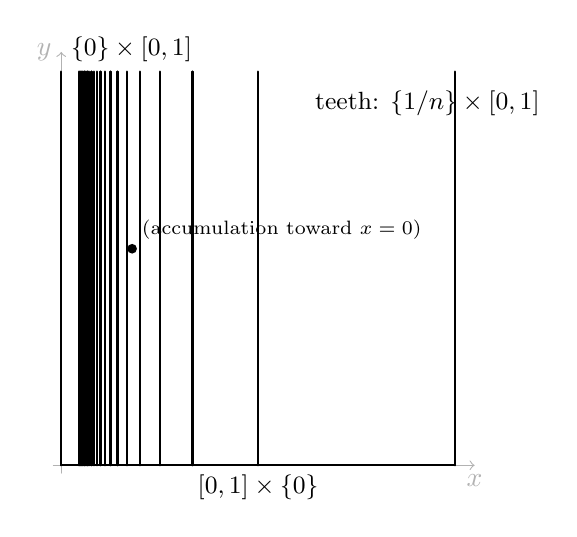
\begin{tikzpicture}[scale=5, line cap=round, line join=round]

  % Axes (optional)
  \draw[->, gray!60] (-0.02,0) -- (1.05,0) node[below] {$x$};
  \draw[->, gray!60] (0,-0.02) -- (0,1.05) node[left] {$y$};

  % Base segment [0,1] x {0}
  \draw[thick] (0,0) -- (1,0);

  % Spine {0} x [0,1]
  \draw[thick] (0,0) -- (0,1);

  % Teeth at x = 1/n, n=1..N
  \def\N{22}
  \foreach \n in {1,...,\N} {
    \pgfmathsetmacro\x{1/(\n)}
    \draw[thick] (\x,0) -- (\x,1);
  }

  % Labels
  \node[above right] at (0,1) {\small $\{0\}\times[0,1]$};
  \node[below] at (0.5,0) {\small $[0,1]\times\{0\}$};

  \node[anchor=west] at (0.62,0.92) {\small teeth: $\{1/n\}\times[0,1]$};

  % Optional: a point showing accumulation near x=0
  \fill (0.18,0.55) circle (0.35pt);
  \node[above right] at (0.18,0.55) {\scriptsize (accumulation toward $x=0$)};

\end{tikzpicture}



